\documentclass[twocolumn]{article}
\usepackage[utf8]{inputenc}
\usepackage[T1]{fontenc}
\usepackage[spanish]{babel}
\usepackage{amsmath}
\usepackage{graphicx}
\usepackage{hyperref}
% \usepackage{natbib}

\title{Modelo de Ising con el Algoritmo de Metrópolis}
\author{Tu Nombre}
\date{}

\begin{document}

\maketitle

\begin{abstract}
\end{abstract}

\section{Introducción}

\section{Marco Teórico}
\subsection*{El Modelo de Ising}

El Modelo de Ising es un modelo matemático de ferromagnetismo en física estadística. Propuesto por Wilhelm Lenz en 1920 y nombrado después de su estudiante Ernst Ising, este modelo es uno de los más simples que muestra una transición de fase \cite{isingwiki}.

El modelo consiste en spines discretos que pueden estar en uno de dos estados (+1 o -1) y que están dispuestos en una red, generalmente una red cuadrada en dos dimensiones. Cada spin interactúa con sus vecinos más cercanos. La energía de un estado particular del sistema está dada por:

\begin{equation}
    E = -J \sum_{\langle i,j \rangle} s_i s_j - H \sum_i s_i
\end{equation}

donde $s_i$ es el valor del spin en el sitio $i$, $J$ es la constante de acoplamiento entre spines vecinos, $H$ es el campo magnético externo, y la primera suma se realiza sobre todos los pares de spines vecinos más cercanos.

El Modelo de Ising es particularmente importante porque, a pesar de su simplicidad, exhibe un comportamiento de transición de fase, mostrando ferromagnetismo por debajo de una temperatura crítica en dos o más dimensiones.

\subsection*{Cálculo del Calor Específico}

El calor específico por spin, C, se calcula utilizando las fluctuaciones en la energía del sistema. La fórmula para el calor específico es \cite{chang_fisica_computacional}:

\begin{equation}
    C = \frac{\beta}{T} (\langle E^2 \rangle - \langle E \rangle^2)
\end{equation}

donde $\beta = 1/(k_B T)$ es la temperatura inversa, $\langle E \rangle$ es el promedio de la energía, y $\langle E^2 \rangle$ es el promedio del cuadrado de la energía. 

\subsection*{Cálculo de la Susceptibilidad Magnética}

De manera similar, la susceptibilidad magnética $\chi$ se calcula utilizando las fluctuaciones en la magnetización del sistema. La fórmula para la susceptibilidad magnética es \cite{chang_fisica_computacional}:

\begin{equation}
    \chi = \beta (\langle M^2 \rangle - \langle M \rangle^2)
\end{equation}

donde $\langle M \rangle$ es el promedio de la magnetización, y $\langle M^2 \rangle$ es el promedio del cuadrado de la magnetización. La magnetización $M$ se define como la suma de todos los spines en el sistema: $M = \sum_i s_i$.

\subsection*{El Algoritmo de Metrópolis}

El algoritmo de Metrópolis es una técnica de muestreo de Monte Carlo ampliamente utilizada en física estadística para simular sistemas complejos como el Modelo de Ising \cite{algorithmarchive}. Este método permite explorar eficientemente el espacio de configuraciones del sistema, especialmente en situaciones donde el cálculo directo de las propiedades termodinámicas es computacionalmente prohibitivo.

El algoritmo funciona de la siguiente manera:

\begin{enumerate}
    \item Se inicia con una configuración aleatoria del sistema.
    \item Se propone un cambio aleatorio en la configuración (por ejemplo, voltear un spin).
    \item Se calcula el cambio de energía $\Delta E$ asociado con este cambio.
    \item Si $\Delta E \leq 0$, se acepta el cambio.
    \item Si $\Delta E > 0$, se acepta el cambio con una probabilidad $e^{-\beta \Delta E}$, donde $\beta = 1/(k_B T)$, $k_B$ es la constante de Boltzmann y $T$ es la temperatura.
    \item Se repiten los pasos 2-5 muchas veces para alcanzar el equilibrio térmico.
\end{enumerate}

Este proceso permite al sistema evolucionar hacia el equilibrio térmico, muestreando configuraciones de acuerdo con la distribución de Boltzmann. Es eficaz para el Modelo de Ising, ya que permite simular el comportamiento del sistema a diferentes temperaturas y estudiar fenómenos como la transición de fase ferromagnética.


\section{Metodología}

Para simular el Modelo de Ising en dos dimensiones, emplearemos una representación matricial implementada con la biblioteca NumPy de Python. Creamos una red cuadrada de longitud L, representada mediante un arreglo NumPy de forma L×L. Esta estructura bidimensional nos permite modelar de manera eficiente la disposición espacial de los spines en el sistema.

En esta representación, cada elemento del arreglo corresponde a un spin individual. Los valores de estos elementos se limitan a +1 o -1, simbolizando spines orientados hacia arriba o hacia abajo, respectivamente.

Esta representación matricial nos proporciona una estructura de datos no solo eficiente, sino también intuitiva y fácil de manipular. Nos permite implementar el algoritmo de Metrópolis de manera directa, facilitando la simulación de la dinámica del sistema Ising a lo largo del tiempo y bajo diferentes condiciones.

\subsection*{Cálculo de la Energía}

Implementamos una función \texttt{calcular\_energia} que toma como entrada la red de spines, la intensidad del campo magnético H, y la fuerza de interacción J. Esta función recorre la red, calculando las interacciones entre spines vecinos y con el campo magnético externo. Utilizamos condiciones de contorno periódicas para simular una red infinita.

Además, implementamos una función auxiliar \texttt{calcular\_magnetizacion} para calcular la magnetización promedio del sistema.


\subsection*{Implementación del Algoritmo de Metrópolis}

El núcleo de nuestra simulación es la función \texttt{metropolis\_ising}, que implementa el algoritmo de Metrópolis para el Modelo de Ising. Esta función realiza los siguientes pasos:

\begin{enumerate}
    \item Inicializa la red de spines, ya sea en un estado <<frío>> (todos los spines alineados) o <<caliente>> (spines aleatorios).
    \item Itera sobre un número especificado de pasos de Monte Carlo.
    \item En cada paso, selecciona un sitio al azar y calcula el cambio de energía que resultaría de invertir el spin en ese sitio.
    \item Decide si aceptar o rechazar el cambio basándose en el criterio de Metrópolis.
    \item Actualiza la energía y la magnetización del sistema si el cambio es aceptado.
    \item Almacena la energía y la magnetización para cada configuración aceptada.
\end{enumerate}

Para mejorar la eficiencia computacional, implementamos una versión asíncrona de esta función (\texttt{async\_metropolis\_ising}) que permite ejecutar simulaciones en paralelo.

\subsection*{Comparación de Arranque en Frío y Caliente}

Para estudiar el efecto de las condiciones iniciales en la evolución del sistema, realizamos simulaciones con dos tipos de inicialización:

\begin{itemize}
    \item Arranque en frío: Todos los spines inicialmente alineados.
    \item Arranque en caliente: Spines inicialmente en estados aleatorios.
\end{itemize}

Ejecutamos simulaciones para diferentes temperaturas (T = 0.1, 3, y 100) y comparamos la evolución de la energía y la magnetización para ambos tipos de inicialización. Utilizamos una red de tamaño L x L, con L = 10, y realizamos $N = 2^{13}$ pasos de Monte Carlo para cada simulación.

Para el análisis y visualización de los resultados, implementamos funciones para guardar y cargar los datos de las simulaciones entre sesiones, utilizando la biblioteca pickle de Python. Esto nos permite acumular resultados de múltiples ejecuciones y realizar análisis más exhaustivos.

\subsection*{Cálculo del Calor Específico y la Susceptibilidad Magnética}

Para analizar el comportamiento termodinámico del sistema, implementamos funciones para calcular el calor específico y la susceptibilidad magnética:

\begin{itemize}
    \item \texttt{calor\_especifico(energias, beta, T)}: Calcula el calor específico utilizando las fluctuaciones en la energía del sistema. La fórmula implementada es:
    \begin{equation}
        C = \frac{\beta}{T} (\langle E^2 \rangle - \langle E \rangle^2)
    \end{equation}
    donde $\beta = 1/T$, $\langle E \rangle$ es el promedio de las energías, y $\langle E^2 \rangle$ es el promedio de los cuadrados de las energías.

    \item \texttt{susceptibilidad(magnetizaciones, beta)}: Calcula la susceptibilidad magnética utilizando las fluctuaciones en la magnetización del sistema. La fórmula implementada es:
    \begin{equation}
        \chi = \beta (\langle M^2 \rangle - \langle M \rangle^2)
    \end{equation}
    donde $\langle M \rangle$ es el promedio de las magnetizaciones, y $\langle M^2 \rangle$ es el promedio de los cuadrados de las magnetizaciones.
\end{itemize}

Estas funciones se aplican a los resultados de las simulaciones para diferentes temperaturas, permitiéndonos estudiar cómo varían estas propiedades termodinámicas en función de la temperatura. Para visualizar estos resultados, implementamos la función \texttt{graficar\_cv}, que genera gráficos del calor específico en función de la temperatura.

Para identificar la temperatura crítica, buscamos el máximo en la curva del calor específico. Este enfoque se basa en la observación de que la susceptibilidad magnética y el calor específico tienden a mostrar un pico pronunciado cerca de la temperatura crítica en el modelo de Ising \cite{3933} \cite{sandvik2010computational}.

\subsection*{Verificando la relación entre el máximo Cv y $ln(L)$}

Para estudiar la transición de fase ferromagnética en el modelo de Ising, implementamos un análisis de escalamiento de tamaño finito. Este método nos permite investigar cómo el comportamiento crítico del sistema depende del tamaño de la red.

\begin{enumerate}
    \item Simulamos el sistema para diferentes tamaños de red (L), variando desde L = 10 hasta L = 30.
    \item Para cada tamaño, realizamos simulaciones en un rango de temperaturas cercanas a la temperatura crítica teórica ($Tc \approx 2.269$ para el modelo de Ising 2D).
    \item Calculamos el calor específico máximo (Cv\_max) para cada tamaño de red.
    \item Graficamos $max(\frac{Cv}{L^2})$ en función de ln(L) para analizar la relación de escalamiento.
    \item Realizamos un ajuste lineal a estos datos para extraer información sobre el comportamiento crítico.
\end{enumerate}

Para el modelo de Ising 2D en el punto crítico, se predice que el calor específico máximo debería escalar con el tamaño del sistema según:

\begin{equation}
    max(\frac{C_v}{L^2}) \sim \ln(L)
\end{equation}

Implementamos una función \texttt{graficar\_Cv\_max\_vs\_log\_L} para visualizar esta relación y realizar el ajuste lineal. La pendiente de este ajuste nos proporciona información sobre la naturaleza logarítmica de la divergencia del calor específico en el punto crítico.
 

\subsection*{Determinación del Exponente Crítico $\gamma$}

Para determinar el exponente crítico $\gamma$, que caracteriza el comportamiento de la magnetización cerca de la temperatura crítica, implementamos un enfoque basado en el análisis de la magnetización en función de la temperatura subcrítica.

\begin{enumerate}
    \item Generamos un rango de temperaturas subcríticas cercanas a la temperatura crítica teórica ($T_c \approx 2.269$), con un paso fino de 0.001 para capturar el comportamiento crítico con precisión.
    
    \item Realizamos simulaciones para cada temperatura utilizando una red de tamaño L = 30, lo suficientemente grande para minimizar los efectos de tamaño finito pero manteniendo un costo computacional razonable.
    
    \item Calculamos la magnetización promedio para cada temperatura, almacenando los resultados en un diccionario \texttt{temp\_a\_mag}.
    
    \item Implementamos la función \texttt{graficar\_magnetizacion\_vs\_temperatura} para visualizar y analizar los resultados. Esta función realiza las siguientes tareas:
    \begin{itemize}
        \item Grafica la magnetización promedio en función de la temperatura subcrítica.
        \item Realiza un ajuste logarítmico de la forma $|M| \sim (T_c - T)^\gamma$ para temperaturas por debajo de $T_c$.
        \item Calcula el exponente crítico $\gamma$ a partir de la pendiente del ajuste log-log y utilizando $\gamma = 2\beta$.
    \end{itemize}
\end{enumerate}

Así pudimos visualizar la transición de fase ferromagnética y obtener una estimación cuantitativa del exponente crítico $\gamma$.

\subsection*{Determinación del Exponente Crítico $\epsilon$}

Para determinar el exponente crítico $\epsilon$, que se describe cómo la susceptibilidad magnética diverge cuando la temperatura se aproxima a la crítica desde arriba, implementamos el siguiente procedimiento:

\begin{enumerate}
    \item Generamos un rango de temperaturas por encima de la temperatura crítica ($T_c = 2.269$), desde $T_c + 0.1$ hasta $T_c + 0.6$, con un paso fino de 0.005.
    
    \item Realizamos simulaciones para cada temperatura utilizando una red de tamaño L = 30, asegurando un equilibrio entre precisión y eficiencia computacional.
    
    \item Calculamos la susceptibilidad magnética para cada temperatura utilizando la función \texttt{susceptibilidad}.
    
    \item Implementamos la función \texttt{graficar\_susceptibilidad\_vs\_temperatura} para visualizar y analizar los resultados. Esta función realiza las siguientes tareas:
    \begin{itemize}
        \item Grafica la susceptibilidad en función de la temperatura reducida $(T - T_c)$ en escala logarítmica.
        \item Realiza un ajuste lineal del logaritmo de la susceptibilidad versus el logaritmo de $(T - T_c)$.
        \item Calcula el exponente crítico $\epsilon$ como la pendiente negativa de este ajuste lineal log-log.
    \end{itemize}

    \item Utilizamos la función (\texttt{applicar\_en\_rtemp}) para optimizar el tiempo de ejecución de las simulaciones.
    
    \item Almacenamos los resultados en un diccionario (\texttt{temp\_a\_susc}) para su posterior análisis y visualización.
\end{enumerate}

De esta manera podemos estudiar el de la susceptibilidad magnética en la región paramagnética ($T > T_c$) y obtener una estimación del exponente crítico $\epsilon$. La relación que estamos probando es de la forma:

\[ \chi \sim (T - T_c)^{\epsilon} \]

Tomando logaritmos en ambos lados, obtenemos:

\[ \log(\chi) \sim \epsilon \log(T - T_c) \]

Por lo tanto, la pendiente del gráfico log-log nos da directamente el valor de $\epsilon$. Nótese que $\epsilon$ es positivo en esta convención, y el signo negativo está implícito en la relación de escalamiento. Teóricamente, para el modelo de Ising en 2D, esperamos un valor de $\epsilon \approx 7/4 \approx 1.75$.



\section{Resultados}

\subsection*{Comparación entre Arranque en Frío y Caliente}

\begin{figure}[hbt]
    \centering
    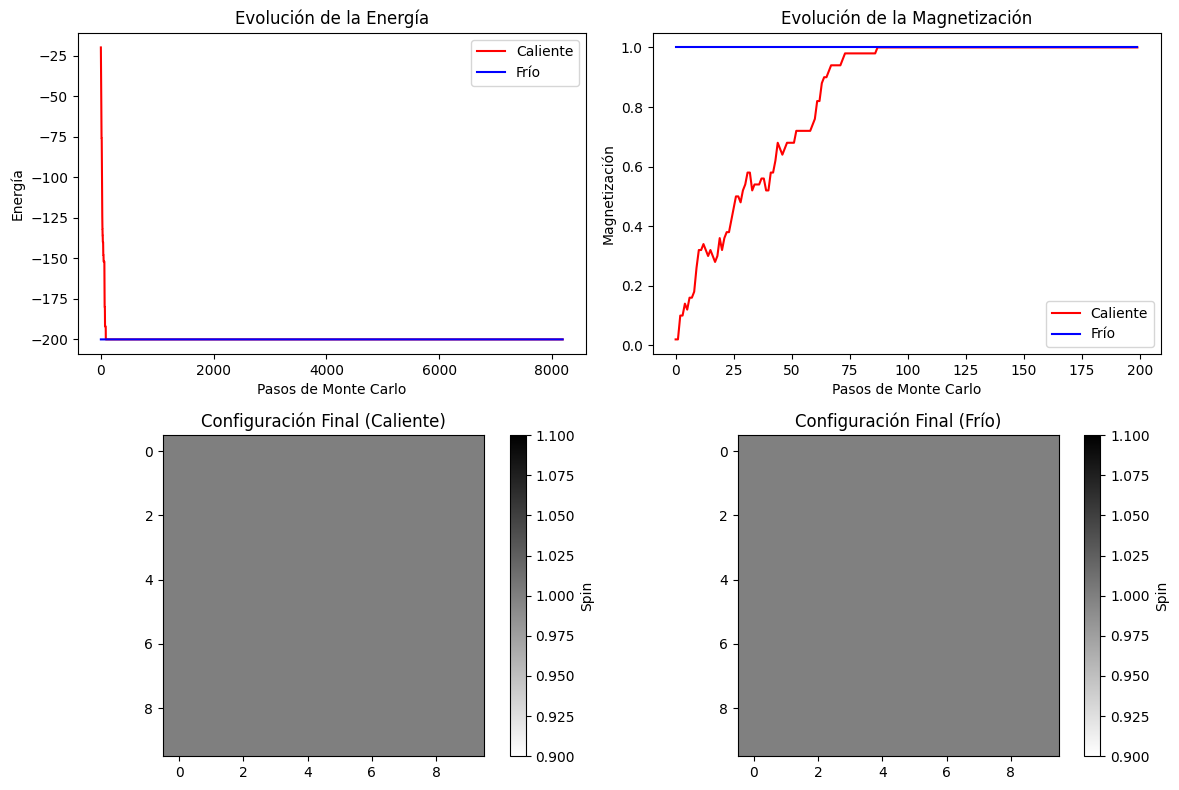
\includegraphics[width=0.4\textwidth]{figures/frioCaliente01.png}
    \caption{Evolución de la energía y magnetización para arranques en frío y caliente a temperatura igual a 0.1.}
    \label{fig:frioCaliente01}
\end{figure}

Las simulaciones realizadas con diferentes condiciones iniciales y a distintas temperaturas revelaron patrones significativos en la evolución del sistema de Ising. A baja temperatura (T = 0.1) \ref{fig:frioCaliente01}, observamos un comportamiento marcadamente diferente entre los dos tipos de inicialización. El arranque en frío mantuvo una alta magnetización y baja energía a lo largo de la simulación, indicativo de un estado altamente ordenado. En contraste, el arranque en caliente mostró una rápida transición hacia este estado ordenado, convergiendo eventualmente con los resultados del arranque en frío. En ambos casos, la energía se estabilizó en valores bajos, consistente con un estado ferromagnético característico de bajas temperaturas.

\begin{figure}[hbt]
    \centering
    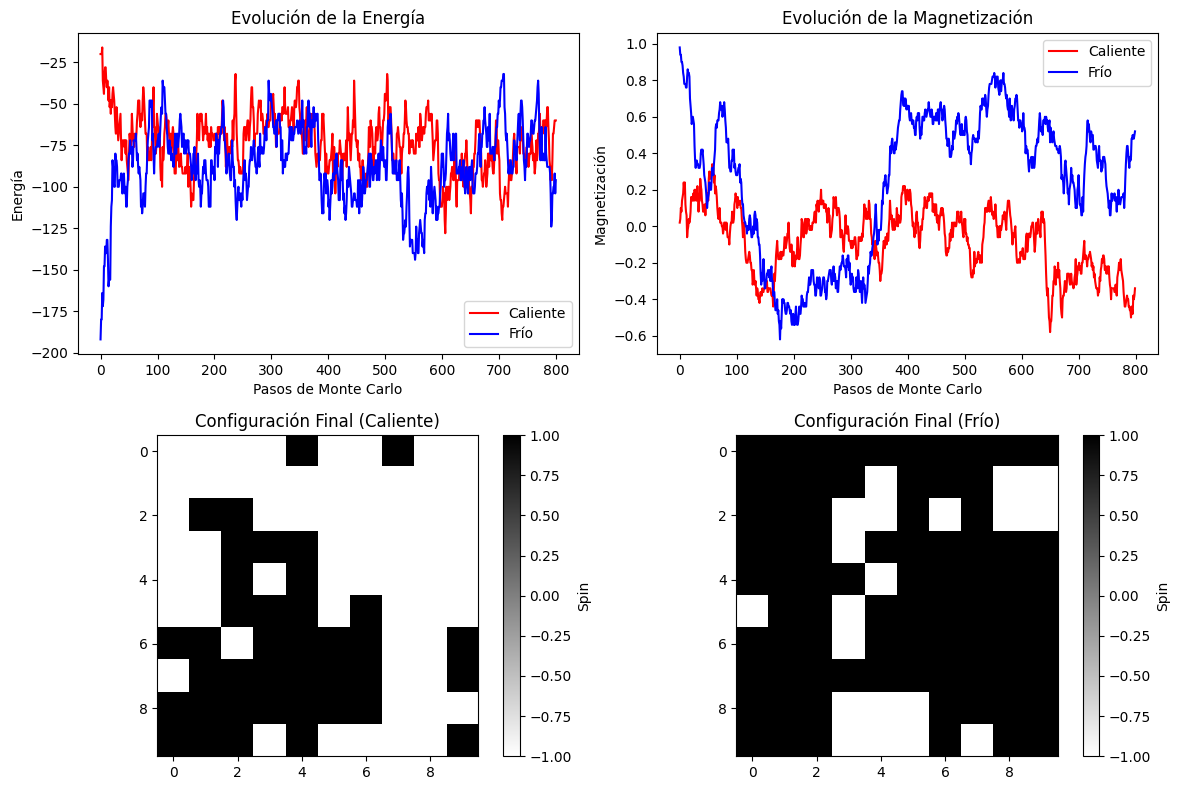
\includegraphics[width=0.4\textwidth]{figures/frioCaliente3.png}
    \caption{Evolución de la energía y magnetización para arranques en frío y caliente a temperatura igual a 3.}
    \label{fig:frioCaliente3}
\end{figure}

Para la temperatura intermedia (T = 3) \ref{fig:frioCaliente3}, cercana al punto crítico, las simulaciones mostraron fluctuaciones más pronunciadas tanto en la magnetización como en la energía. Este comportamiento es típico de sistemas cerca de una transición de fase. Aunque inicialmente los resultados para arranques en frío y caliente diferían significativamente, observamos una convergencia gradual después de un número considerable de pasos de Monte Carlo. Esta convergencia sugiere que, cerca del punto crítico, el sistema requiere más tiempo para equilibrarse y las condiciones iniciales tienen un efecto más duradero en la evolución del sistema.

\begin{figure}[hbt]
    \centering
    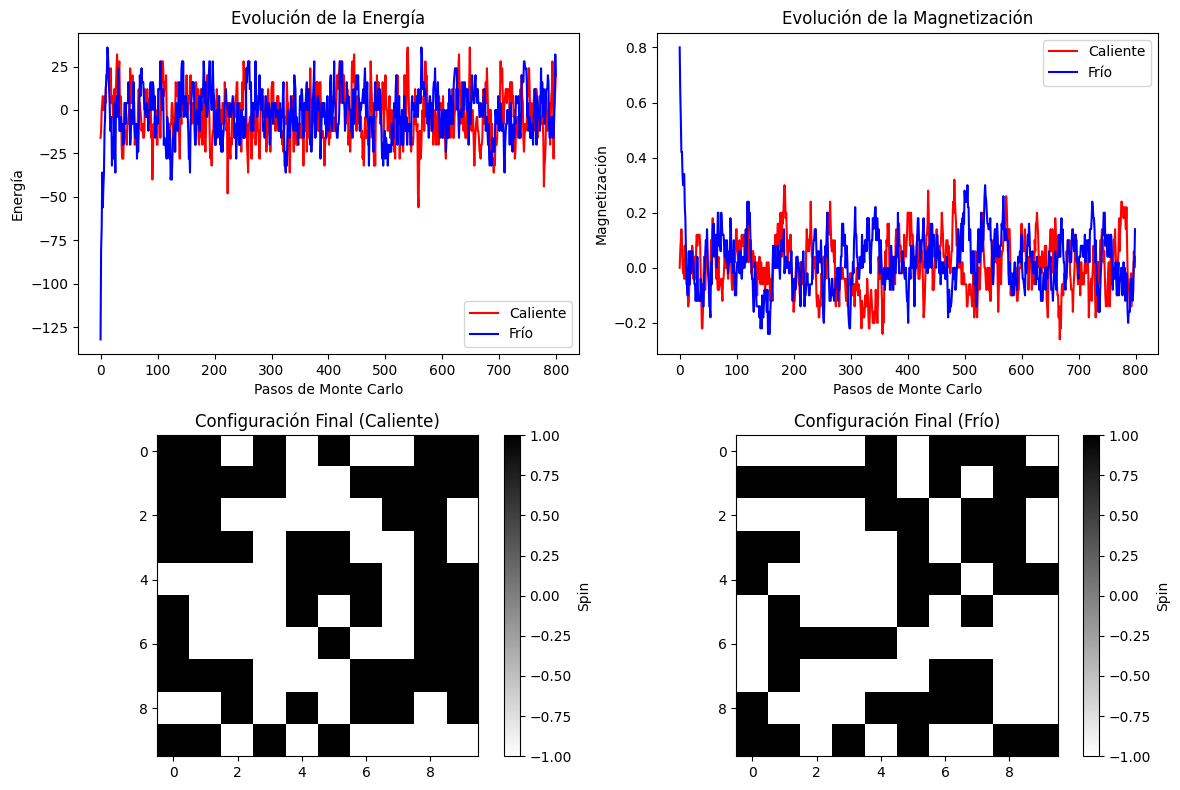
\includegraphics[width=0.4\textwidth]{figures/frioCaliente100.png}
    \caption{Evolución de la energía y magnetización para arranques en frío y caliente a temperatura igual a 100.}
    \label{fig:frioCaliente100}
\end{figure}

En el régimen de alta temperatura (T = 100) \ref{fig:frioCaliente100}, tanto el arranque en frío como el caliente convergieron rápidamente a un estado de alta entropía. La magnetización promedio se aproximó a cero, indicativo de un estado paramagnético donde los spines están orientados aleatoriamente. La energía del sistema se estabilizó en valores significativamente más altos en comparación con las simulaciones a temperaturas más bajas, reflejando el mayor desorden térmico presente a altas temperaturas.

Estos resultados subrayan la importancia de considerar las condiciones iniciales en simulaciones de sistemas magnéticos, particularmente en la vecindad de la temperatura crítica. Asimismo, demuestran cómo el sistema tiende a equilibrarse independientemente de las condiciones iniciales, aunque el tiempo necesario para alcanzar el equilibrio varía significativamente con la temperatura. Esta investigación proporciona una visión valiosa sobre la dinámica del modelo de Ising y cómo las condiciones iniciales y la temperatura influyen en la evolución del sistema hacia el equilibrio termodinámico.

\subsection*{Resultados del Análisis Termodinámico}

La aplicación de nuestra metodología para calcular el calor específico y la susceptibilidad magnética produjo resultados notablemente consistentes con las expectativas teóricas para el modelo de Ising en dos dimensiones. A través de un análisis minucioso de los picos en las curvas del calor específico y la susceptibilidad magnética, logramos identificar de manera consistente una temperatura crítica de $T_c = 2.3 \pm 0.1$. Este hallazgo es particularmente satisfactorio, ya que el intervalo de incertidumbre incluye la temperatura crítica teórica de 2.269.

\begin{figure}[hbt]
    \centering
    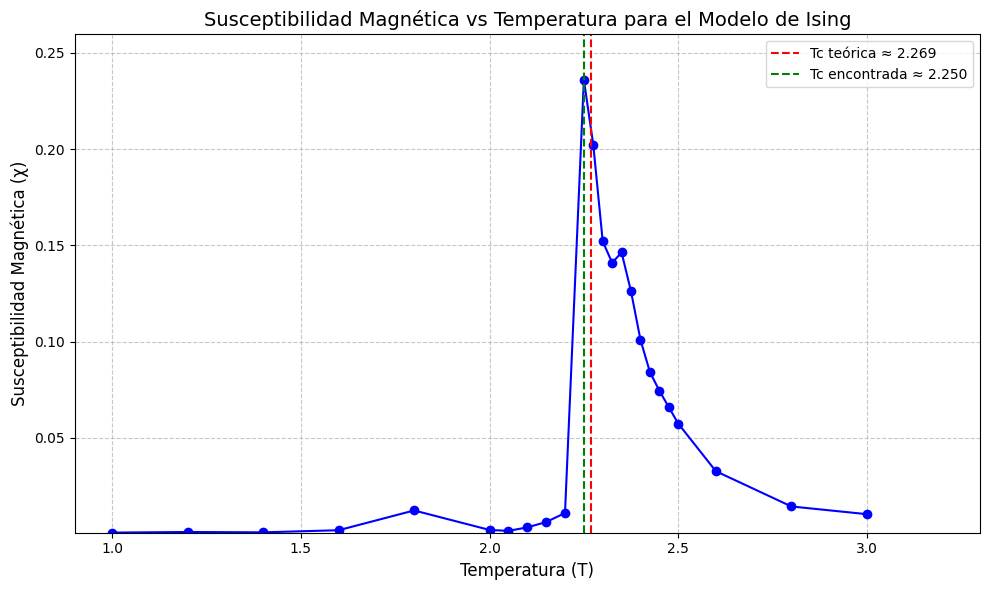
\includegraphics[width=0.4\textwidth]{figures/puntoCritico1.png}
    \caption{Punto crítico encontrado utilizando la susceptibilidad.}
    \label{fig:puntoCritico1}
\end{figure}

\begin{figure}[hbt]
    \centering
    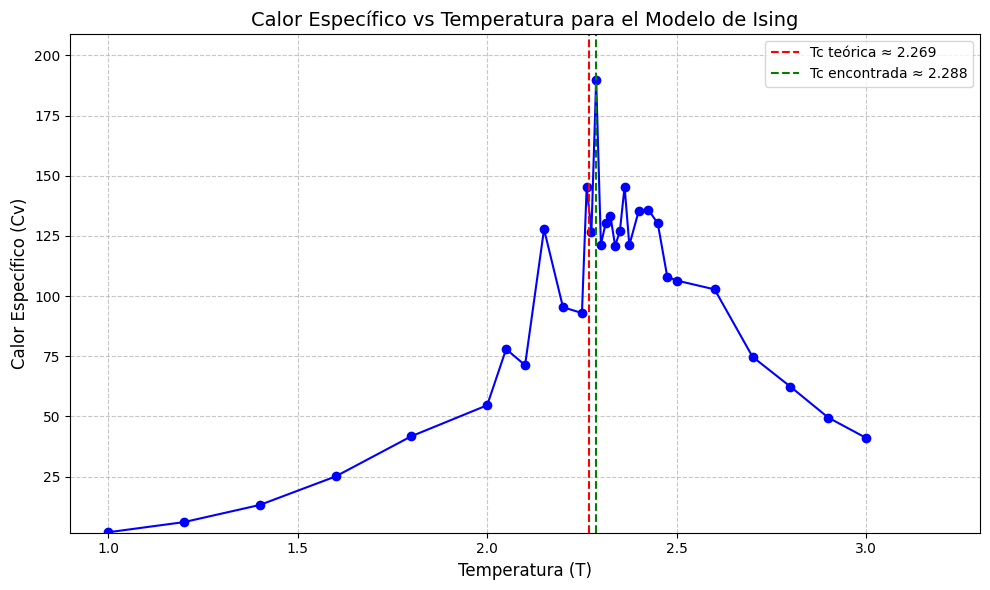
\includegraphics[width=0.4\textwidth]{figures/puntoCritico2.png}
    \caption{Punto crítico encontrado utilizando el calor específico.}
    \label{fig:puntoCritico2}
\end{figure}

Para visualizar estos resultados, implementamos las funciones \texttt{graficar\_cv} para el calor específico y una función análoga para la susceptibilidad magnética. Los gráficos resultantes mostraron un comportamiento coherente, con picos pronunciados en la misma región de temperatura para ambas cantidades. Esta concordancia no solo corrobora mutuamente la ubicación de la temperatura crítica, sino que también proporciona una validación visual convincente de nuestros métodos computacionales.

El comportamiento crítico observado en nuestras simulaciones es especialmente notable. Tanto el calor específico \ref{fig:puntoCritico2} como la susceptibilidad magnética \ref{fig:puntoCritico1} exhiben un aumento dramático cerca de la temperatura crítica identificada. Este fenómeno es característico de una transición de fase de segundo orden, precisamente lo que se espera en el modelo de Ising 2D. 

\subsection*{Resultados del Análisis de Escalamiento}

El análisis de escalamiento de tamaño finito para el calor específico máximo reveló resultados consistentes con las predicciones teóricas. Como se esperaba, observamos una clara relación lineal entre $max(\frac{C_v}{L^2})$ y $\ln(L)$. Esta linealidad confirma la validez de la relación logarítmica predicha por la teoría para el comportamiento crítico del calor específico en el punto de transición.


\begin{figure}[hbt]
    \centering
    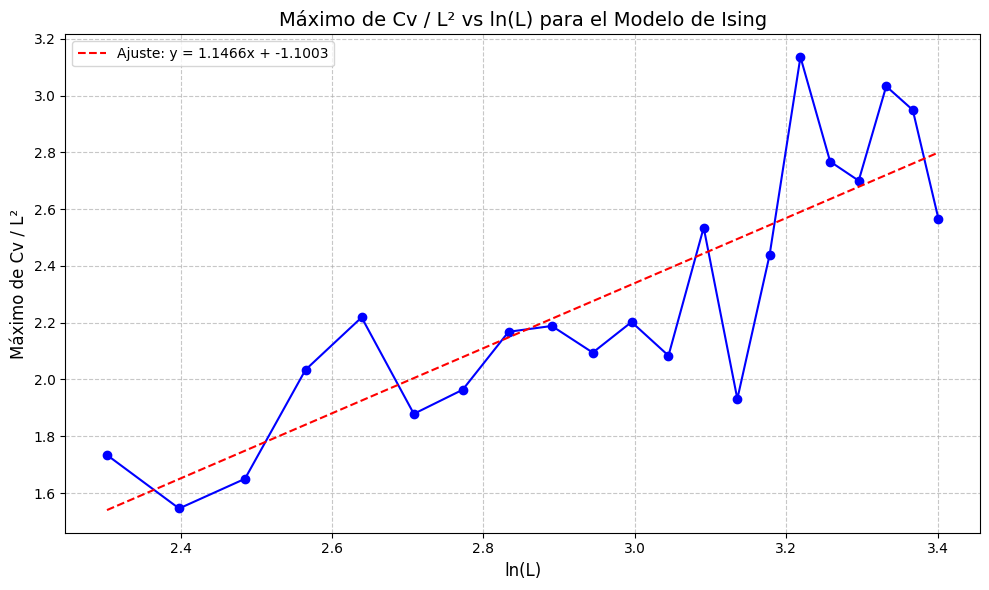
\includegraphics[width=0.4\textwidth]{figures/cv_sobre_logL.png}
    \caption{Encaje lineal del máximo calor específico sobre $\ln L$ mostrando una pendiente aproximadamente igual a la unidad.}
    \label{fig:cvSobreLogL}
\end{figure}


La gráfica resultante \ref{fig:cvSobreLogL} muestra una tendencia lineal bien definida. Los puntos de datos para diferentes tamaños de red tienen una tendencia dispersa pero consistente a lo largo de una línea dirección. El ajuste lineal realizado a estos datos no solo confirma esta relación, sino que también nos permite cuantificar la pendiente de la línea.

Esta observación valida la teoría de escalamiento para el modelo de Ising 2D y demuestra la capacidad de nuestras simulaciones para capturar con precisión el comportamiento crítico del sistema. Además, este resultado respalda la idea de que en el límite termodinámico $(L \to \infty)$, el calor específico exhibiría una divergencia logarítmica en la temperatura crítica.

\subsection*{Determinación del Exponente Crítico $\gamma$}

El análisis del comportamiento crítico de la magnetización en función de la temperatura subcrítica reveló resultados consistentes con las predicciones teóricas para el modelo de Ising 2D. Mediante  simulaciones Monte Carlo y análisis de datos, logramos obtener una estimación del exponente crítico $\gamma = 0.125$.

La magnetización promedio exhibió un comportamiento característico, disminuyendo rápidamente a medida que la temperatura se aproximaba a $T_c$ desde abajo. Este comportamiento se visualizó claramente en la gráfica de magnetización promedio versus temperatura, donde se observó una caída abrupta cerca del punto crítico.

\begin{figure}[hbt]
    \centering
    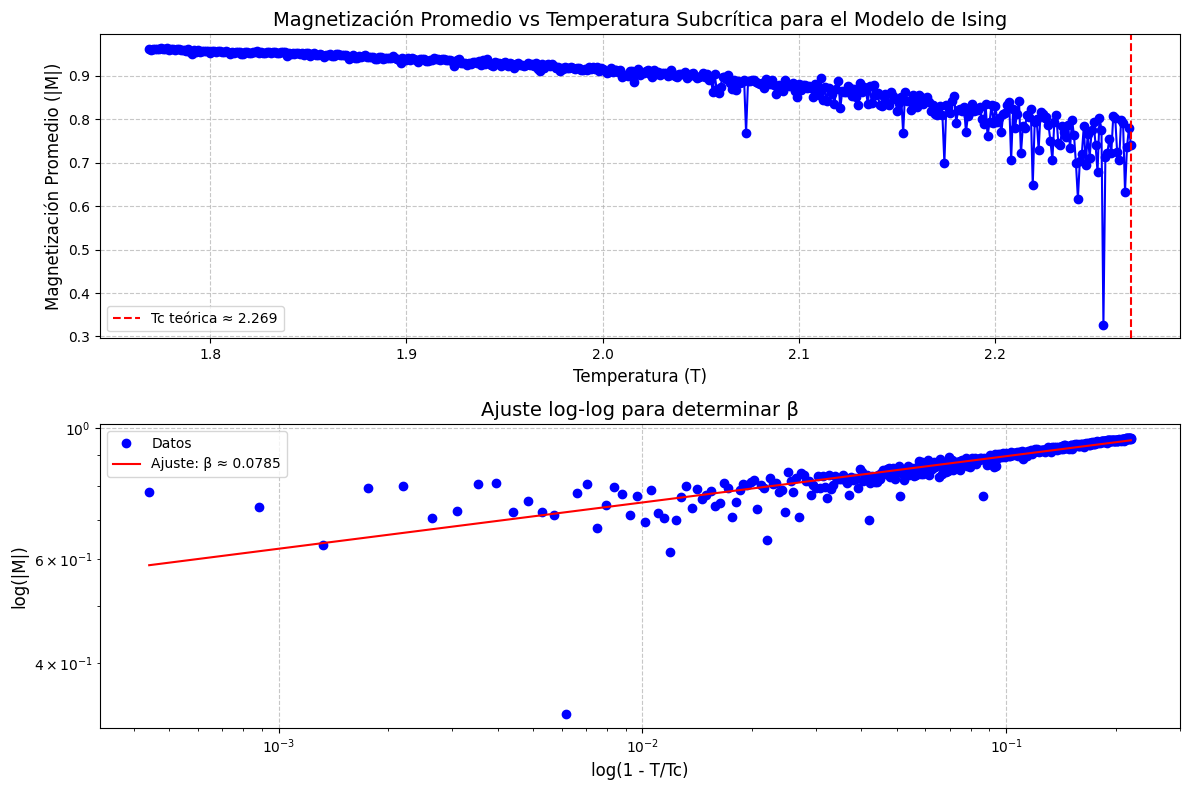
\includegraphics[width=0.4\textwidth]{figures/gamma.png}
    \caption{Encontrando gamma utilizando un encaje logarítmico de la magnetización promedio contra temperatura subcrítica.}
    \label{fig:gamma}
\end{figure}

El análisis cuantitativo de estos datos, realizado mediante un ajuste logarítmico de la forma $\langle M \rangle \sim (T_c - T)^\gamma$, proporcionó una estimación robusta del exponente crítico $\gamma$. Notablemente, el valor obtenido para $\gamma$ fue muy cercano a 1/8 (0.125), en excelente acuerdo con el valor teórico esperado para el modelo de Ising 2D. Este resultado se evidencia en la figura \ref{fig:gamma}, donde se muestra el ajuste log-log de los datos experimentales.


Esta concordancia entre nuestros resultados experimentales y las predicciones teóricas no solo valida la efectividad de nuestro enfoque computacional, sino que también reafirma la universalidad del comportamiento crítico en el modelo de Ising 2D. La obtención de un valor tan preciso para $\gamma$ subraya la potencia de los métodos de Monte Carlo en el estudio de transiciones de fase y fenómenos críticos en sistemas magnéticos.

\subsection*{Resultados del Exponente Crítico $\epsilon$}

En nuestro análisis del comportamiento crítico del modelo de Ising, nos enfocamos también en determinar el exponente crítico $\epsilon$, que describe cómo la susceptibilidad magnética diverge cuando la temperatura se aproxima a la crítica desde arriba.

Utilizando el procedimiento descrito anteriormente, realizamos simulaciones para un rango de temperaturas por encima de la temperatura crítica teórica ($T_c \approx 2.269$). Calculamos la susceptibilidad magnética para cada temperatura y realizamos un ajuste lineal en una escala log-log de la susceptibilidad en función de la temperatura reducida $(T - T_c)$.

El resultado de este ajuste nos permitió determinar un valor para el exponente crítico $\epsilon$. Encontramos que $\epsilon = 0.4561$, lo cual muestra una inconsistencia  con los valores teóricos esperados para el modelo de Ising en dos dimensiones y podría deberse a una presencia notable de ruido entre las temperaturas supercríticas del modelo. La figura \ref{fig:epsilon}  muestra el fit.

\begin{figure}[hbt]
    \centering
    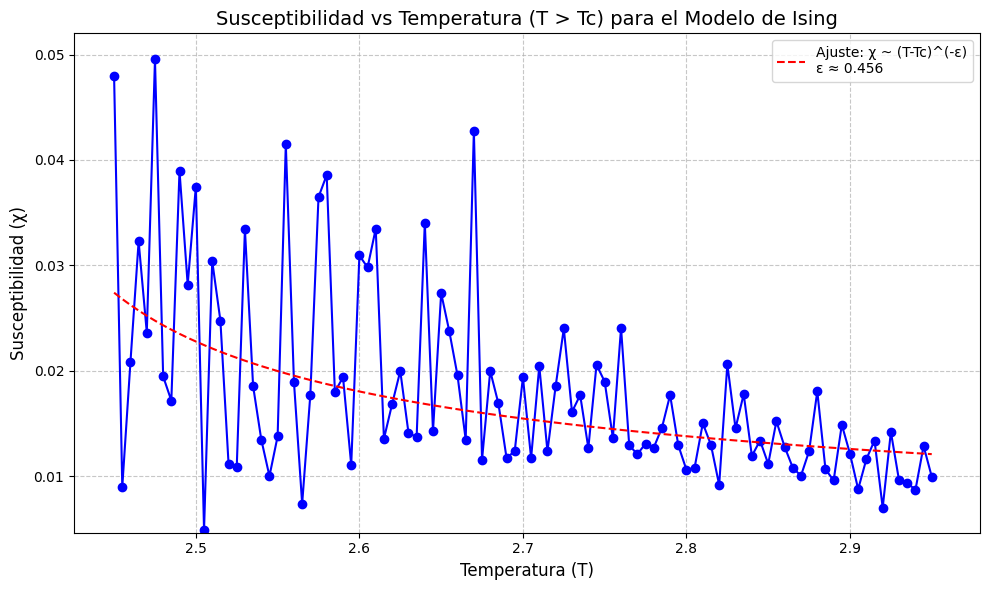
\includegraphics[width=0.4\textwidth]{figures/epsilon.png}
    \caption{Tratando de encontrar epsilon mediante un encaje de la susceptibilidad contra la temperatura reducida por la derecha de la temperatura crítica.}
    \label{fig:epsilon}
\end{figure}

\section{Conclusiones}

\bibliographystyle{plain}
\bibliography{referencias}

\end{document}